\documentclass{beamer}
\usepackage[utf8]{inputenc}
\usepackage{default}
\usepackage{listings}
\usepackage{relsize}
\usepackage{graphicx}
\usepackage{multimedia}

\mode<presentation>{ \usetheme{Singapore} }
\title{ Palestra com nome engraçadinho pra chamar gente }
\subtitle{ A construção do Caos }
\author{ Tomaz Canabrava }

\AtBeginSection[]
{
   \begin{frame}
       \frametitle{Outline}
       \tableofcontents[currentsection]
   \end{frame}
}

\begin{document}
\begin{frame} \titlepage \end{frame}

\begin{frame} \frametitle{1940}
    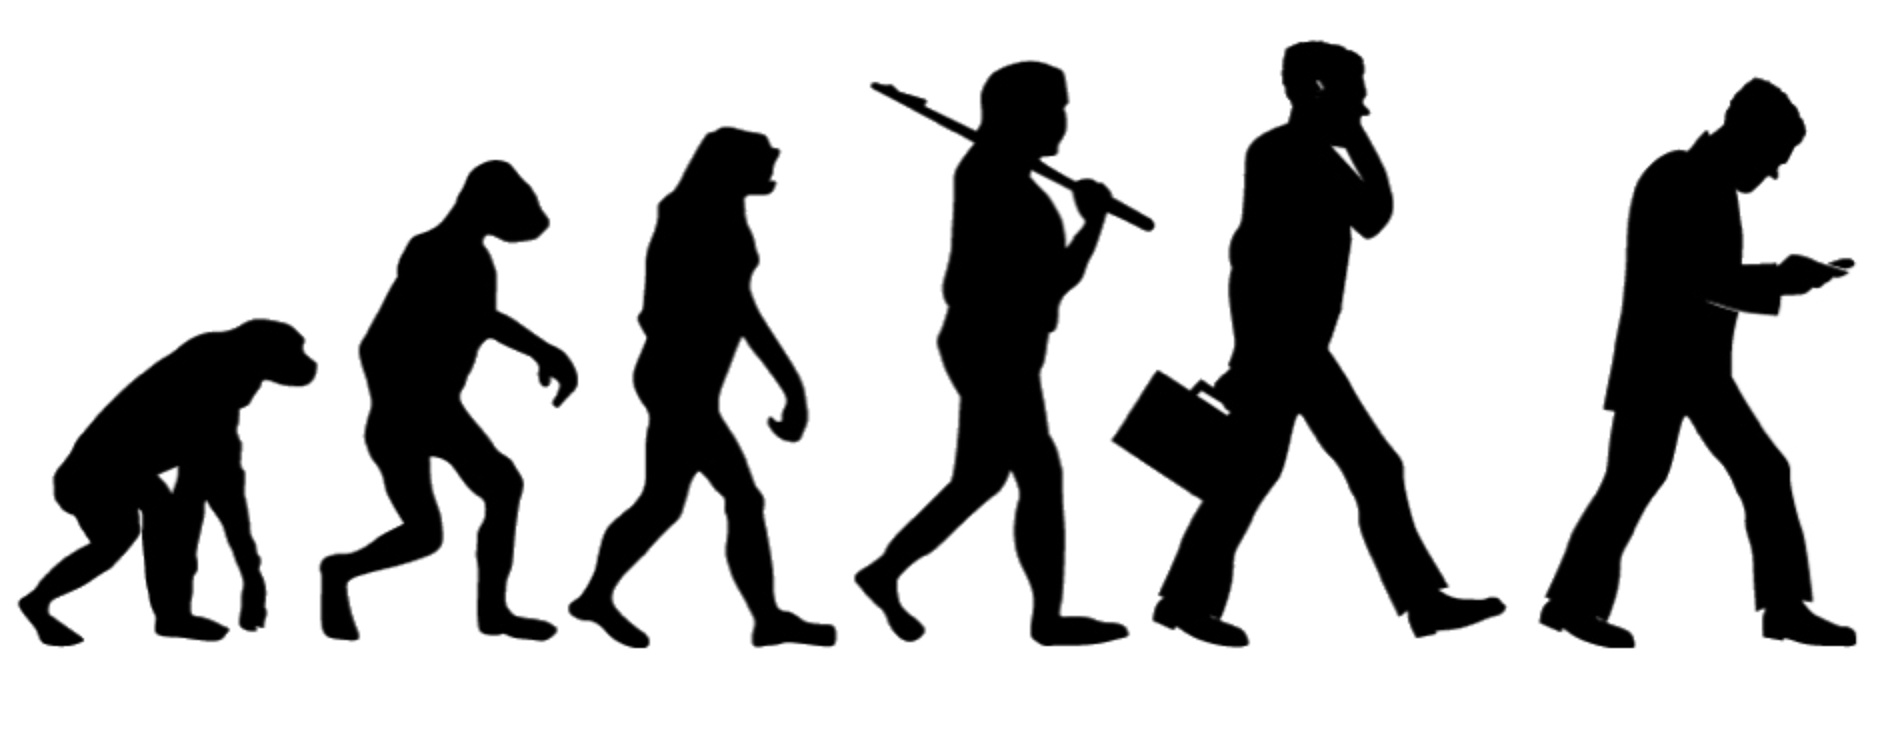
\includegraphics[width=300px]{images/evolution}
\end{frame}

\begin{frame} \frametitle{Invenções Pré-históricas}
    \begin{itemize}
     \item Fogo
     \item Roda
     \item Imprensa
     \pause
     \item Eniac
    \end{itemize}
\end{frame}

\begin{frame} \frametitle{Eniac}
    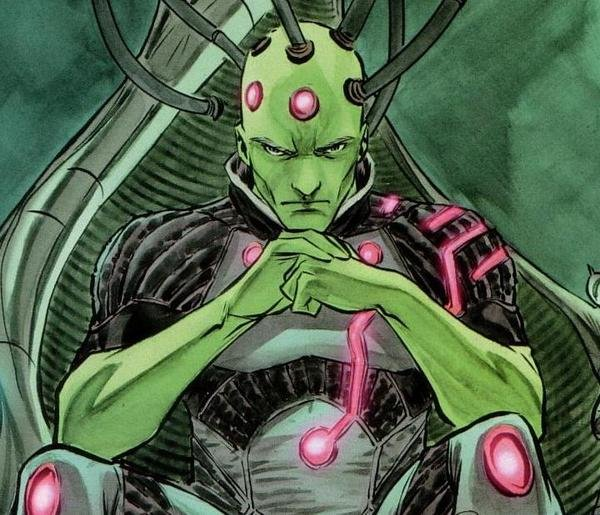
\includegraphics[width=300px]{images/eniac}
\end{frame}

\begin{frame} \frametitle{Eniac em 1940}
    \begin{columns}
    \column{0.5\textwidth}
    \begin{itemize}
        \item Base 10
        \pause
        \item 5000 calculos por segundo
        \pause
        \item 5 Milhões pontos de solda manuais
        \pause
        \item 150kw de energia
        \pause
        \item Não cabia no seu bolso.
    \end{itemize}
    \end{columns}
\end{frame}

\begin{frame} \frametitle{Uma olhada em 150kw}
    \begin{itemize}
    \item 3750 lampadas de 40w
    \item Carregar 150 Androids por um Ano
    \item Um Laser Militar (Ainda em Construção)
    \end{itemize}
\end{frame}

\begin{frame} \frametitle{IBM}
    \begin{columns}
        \column{0.5\textwidth}
        ``I think there is a world market for about five computers''

        Thomas J Watson
        \pause
        \column{0.5\textwidth}
        ``Eu acho que existe um mercado mundial para uns cinco computadores''
    \end{columns}
\end{frame}

\begin{frame} \frametitle{1960 e MainFrames}
    \begin{columns}
        \column{0.5\textwidth}
        \begin{itemize}
            \item Transistores
            \item Módulos de Fita
            \item Cartões Perfurados
            \item ``Super computadores''
            \item Terminais burros
            \item Fortran
        \end{itemize}
        \column{0.5\textwidth}
            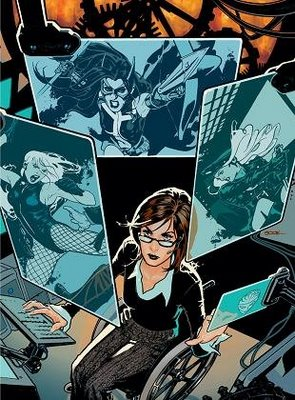
\includegraphics[width=150px]{images/oraculo}
    \end{columns}
\end{frame}

\begin{frame} \frametitle{Fortran}
 \center{“I don't know what the language of the year 2000 will look like, but I know it will be called Fortran.”}
 \linebreak
 \linebreak
 Tony Hoare, ganhador do troféu Turing
 \pause
 \linebreak
 \center{“Não sei como será a linguagem mais usada nos anos 2000, mas sei que ela se chamará fortran.”}
\end{frame}

\begin{frame} \frametitle{Fortran}
    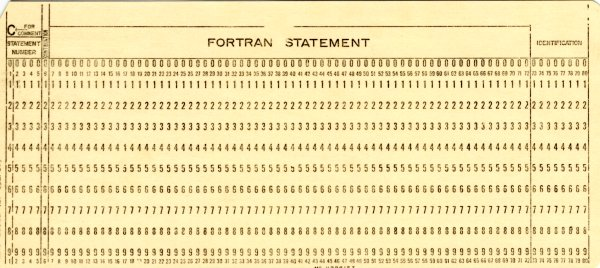
\includegraphics[width=300px]{images/fortran}
\end{frame}

\begin{frame} \frametitle{C e Unix}
    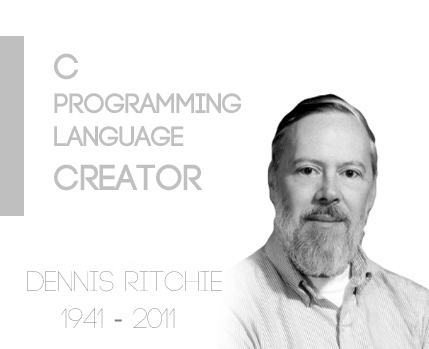
\includegraphics[width=250px]{images/c-unix-creator}
\end{frame}

\begin{frame} \frametitle{ 1980 - 2000, Era dos PC's}
    \begin{itemize}
     \item Menos Potentes
     \item Menos Memória
     \item Menos gastos com Energia
     \item Menos custos de manutenção
     \item ``Pessoais''
     \item 15 diskettes e 99 dolares
    \end{itemize}
\end{frame}

\begin{frame} \frametitle{Windows 3.11}
    \movie[width=300px,height=210px,poster,showcontrols]{}{videos/ballmer-sells-windows.avi}
\end{frame}

\begin{frame}
     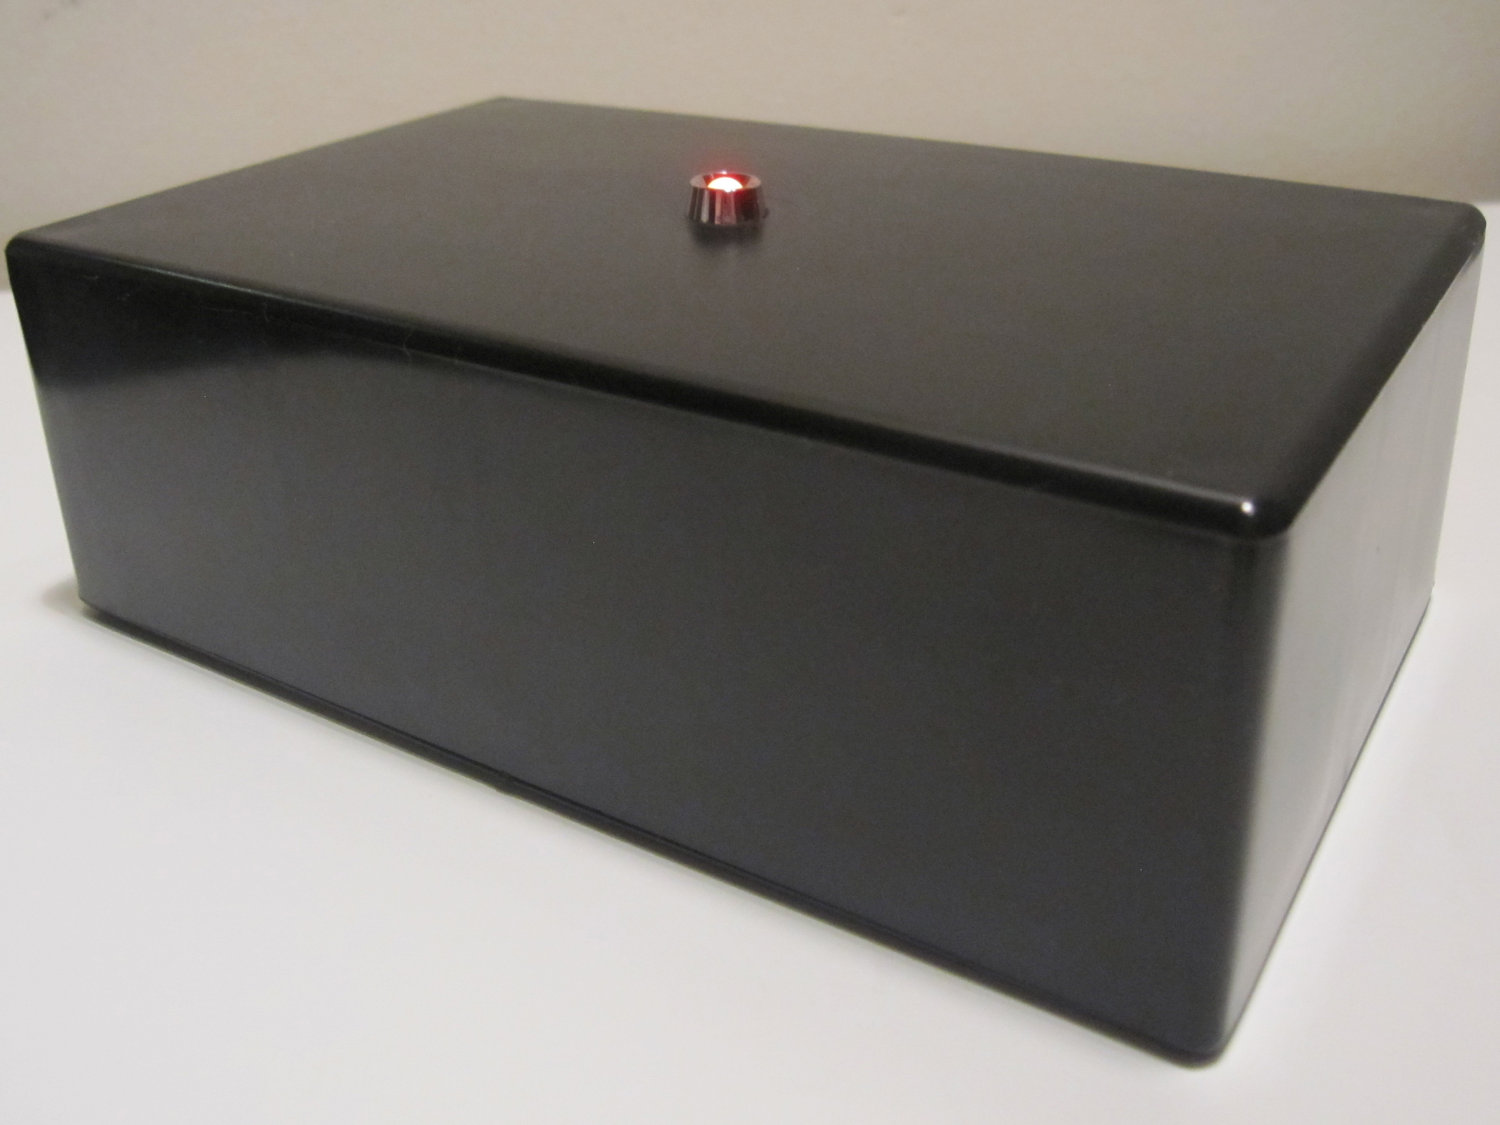
\includegraphics[width=300px]{images/the-internet}
\end{frame}

\begin{frame} \frametitle{A Internet}
     \begin{itemize}
      \item mIRC
      \item icq
      \item netscape
      \item emails
      \item jogos
      \item National Center for Supercomputing Applications
     \end{itemize}
\end{frame}

\begin{frame}
     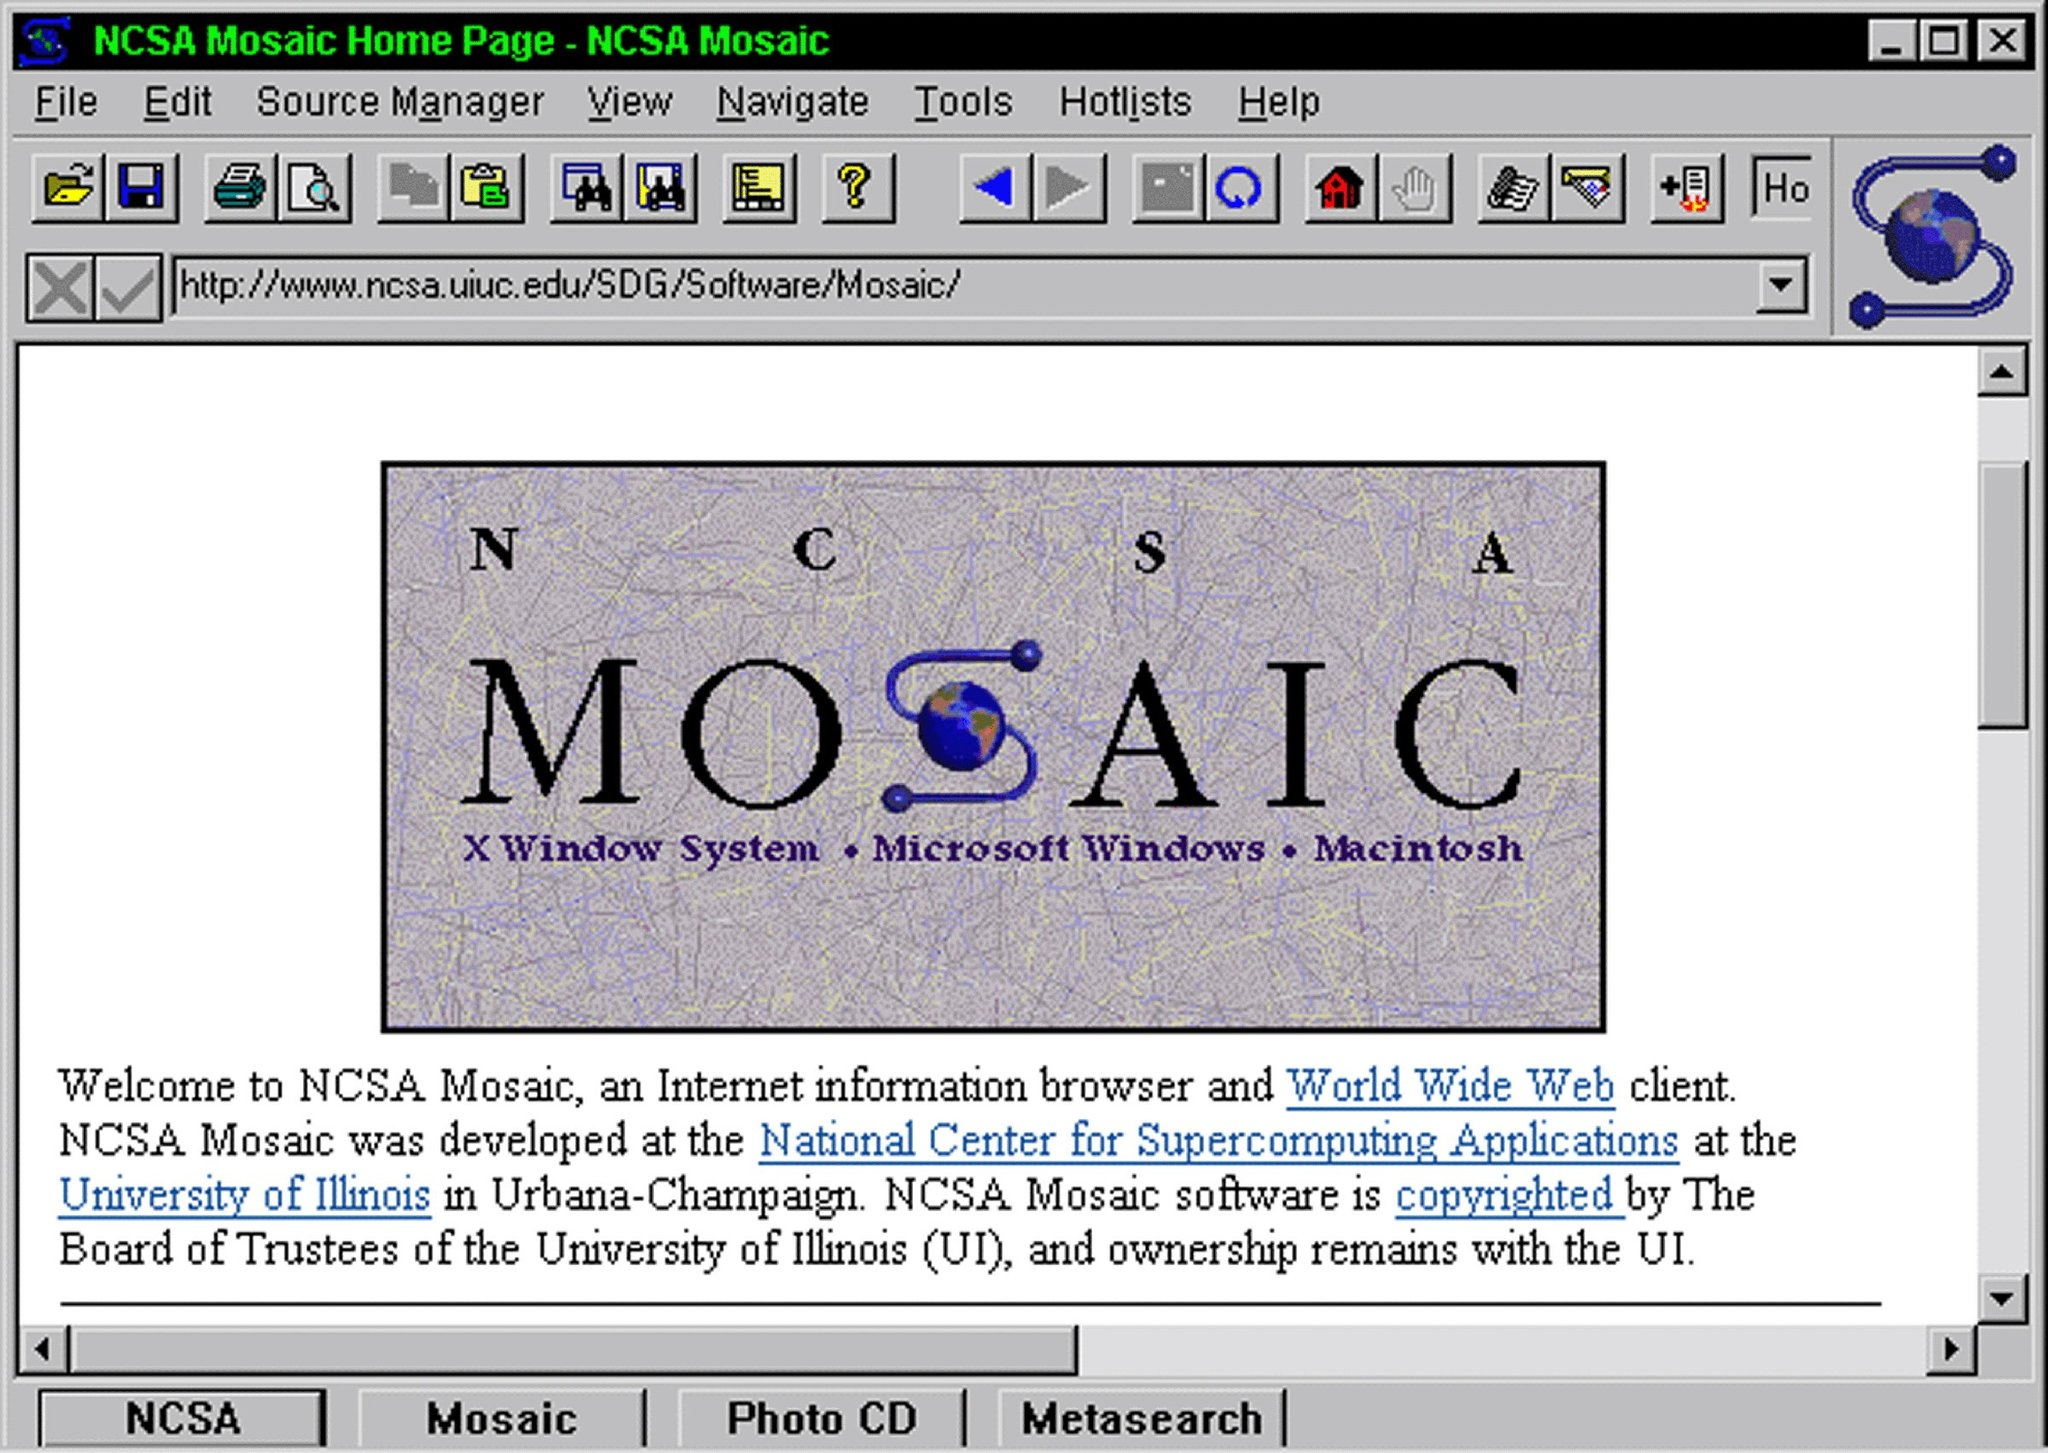
\includegraphics[width=300px]{images/mosaic}
\end{frame}

\begin{frame} \frametitle{Guerra dos Browsers}
    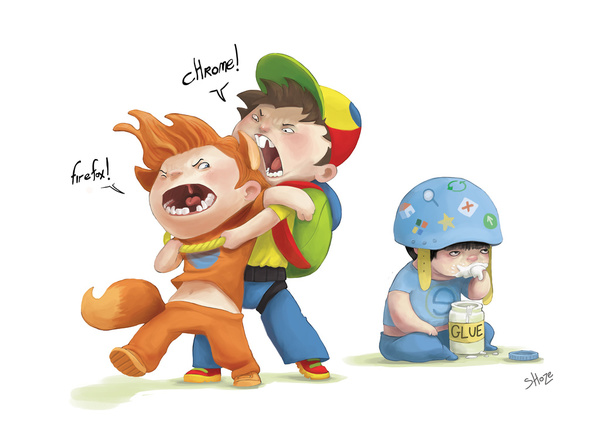
\includegraphics[width=300px]{images/browser-war}
\end{frame}

\begin{frame} \frametitle{Guerra dos Browsers}
    \begin{columns}
        \column{0.5\textwidth}
        \begin{itemize}
            \item Netscape Navigator
            \item Internet Explorer
            \item Opera
            \item Chrome
            \item Firefox
        \end{itemize}
    \end{columns}
\end{frame}

\begin{frame} \frametitle{Guerra dos Browsers}
    \center{O Ganhador? Webkit}
    \begin{itemize}
     \item konqueror
     \item safari
     \item chrome
     \item opera
    \end{itemize}
\end{frame}

\begin{frame}
    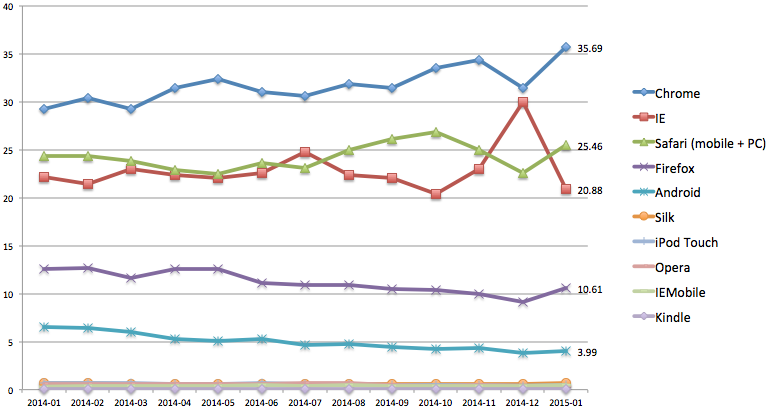
\includegraphics[width=300px]{images/browser-usage}
\end{frame}

\begin{frame} \frametitle{The Cloud}
    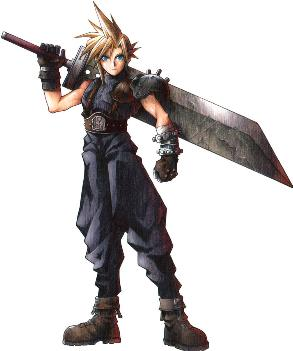
\includegraphics[width=300px]{images/cloud-striffe}
\end{frame}

\end{document}
